%----------------------------------------------------------------------------
\label{STIRAP ridge section}
%----------------------------------------------------------------------------
%----------------------------------------------------------------------------
%----------------------------------------------------------------------------
\begin{figure}
\begin{center}
\leavevmode
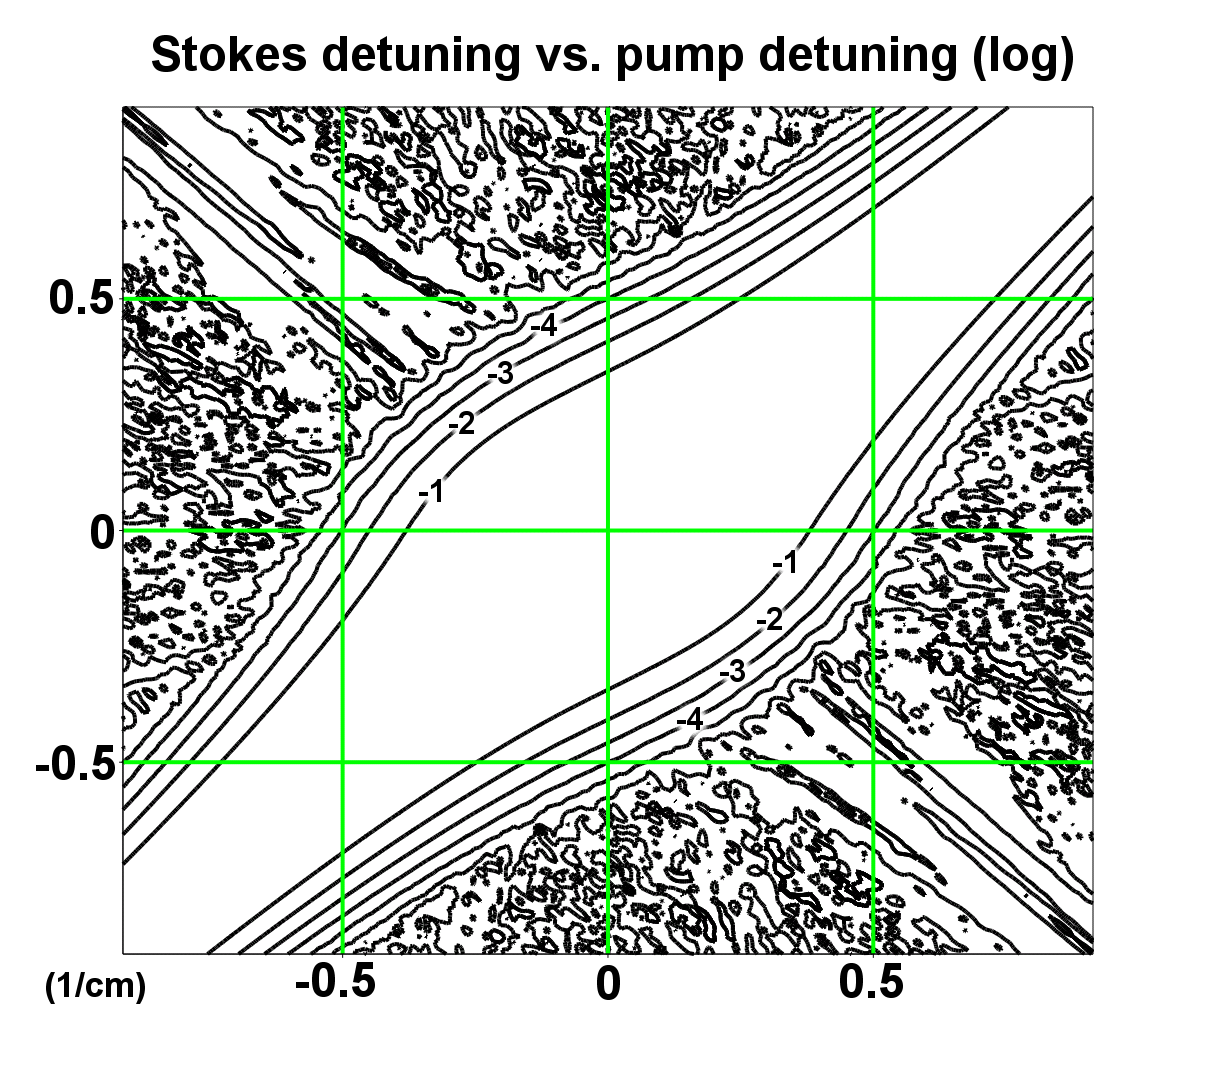
\includegraphics[width=4in]
{ridge/ridge.png}\\
\end{center}
\caption[STIRAP detuning ridge]{STIRAP detuning ridge - The log of the inversion probability is plotted here. See Figure \ref{sp_detuning} for the definition of the Stokes pulse and the pump pulse.}
\label{ridge}
\end{figure} 
%----------------------------------------------------------------------------

%----------------------------------------------------------------------------
%bb defines the bounding box for the pdf
%viewport defines the area of the pdf used
%in sidewaysfigure the last entry in bb moves the caption toward/away the pic
%in sidewaysfigure the second entry in bb moves the pic toward/away the caption
%----------------------------------------------------------------------------
\begin{figure}
\scalebox{0.8}[0.8]{
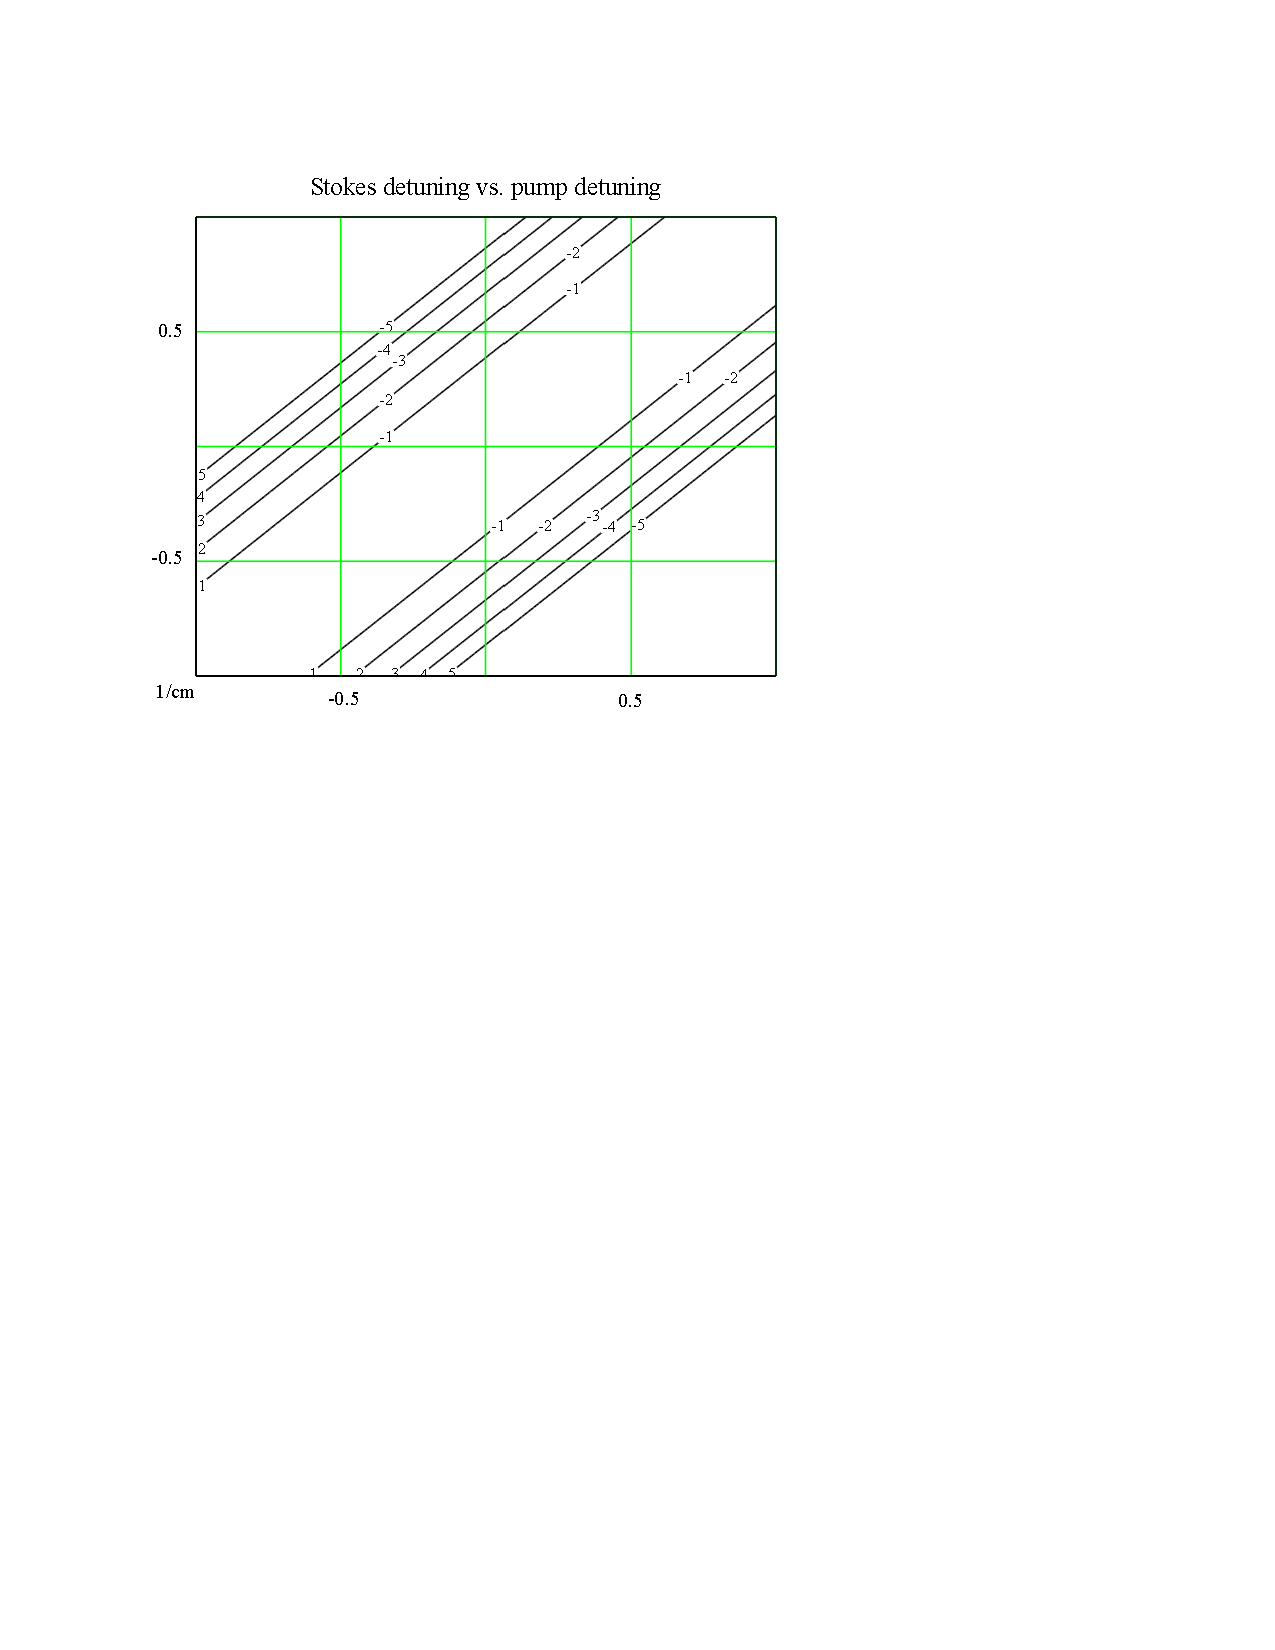
\includegraphics[bb=-30 430 489 700]
{ridge_fit/ridge_fit.pdf}
}
\caption[STIRAP detuning ridge fit]{STIRAP detuning ridge fit - The log of the inversion probability is plotted here.}
\label{ridge_fit}
\end{figure}
%----------------------------------------------------------------------------

%----------------------------------------------------------------------------
The STIRAP process has a unique ``detuning'' feature very different from the corresponding feature for two sequential $\pi$--pulses. The single $\pi$--pulse detuning curve is a sinusoid modulated by a relatively wide Lorentzian (see Section \ref{doppler section}) . The FWHM of this Lorentzian is half the Rabi frequency or, in order to beat the relaxation effects in atmospheric conditions, about one half GHz. This is on the order of the Doppler broadening, so for this discussion, the overall Lorentzian width of a single $\pi$--pulse is near 0.03 inverse cm. To obtain the two $\pi$--pulse detuning line shape we plot the surface formed by the inversion probability as a function of the first pulse (Stokes) detuning and the second pulse (pump) detuning and we get a Lorentzian ``mountain'' with a rough FWHM of 0.03 inverse cm (see Figure \ref{sp_detuning} for the definition of the Stokes pulse and the pump pulse).
%----------------------------------------------------------------------------
%----------------------------------------------------------------------------
%bb defines the bounding box for the pdf
%viewport defines the area of the pdf used
%in sidewaysfigure the last entry in bb moves the caption toward/away the pic
%in sidewaysfigure the second entry in bb moves the pic toward/away the caption
%----------------------------------------------------------------------------
\begin{figure}
\scalebox{0.6}[0.6]{
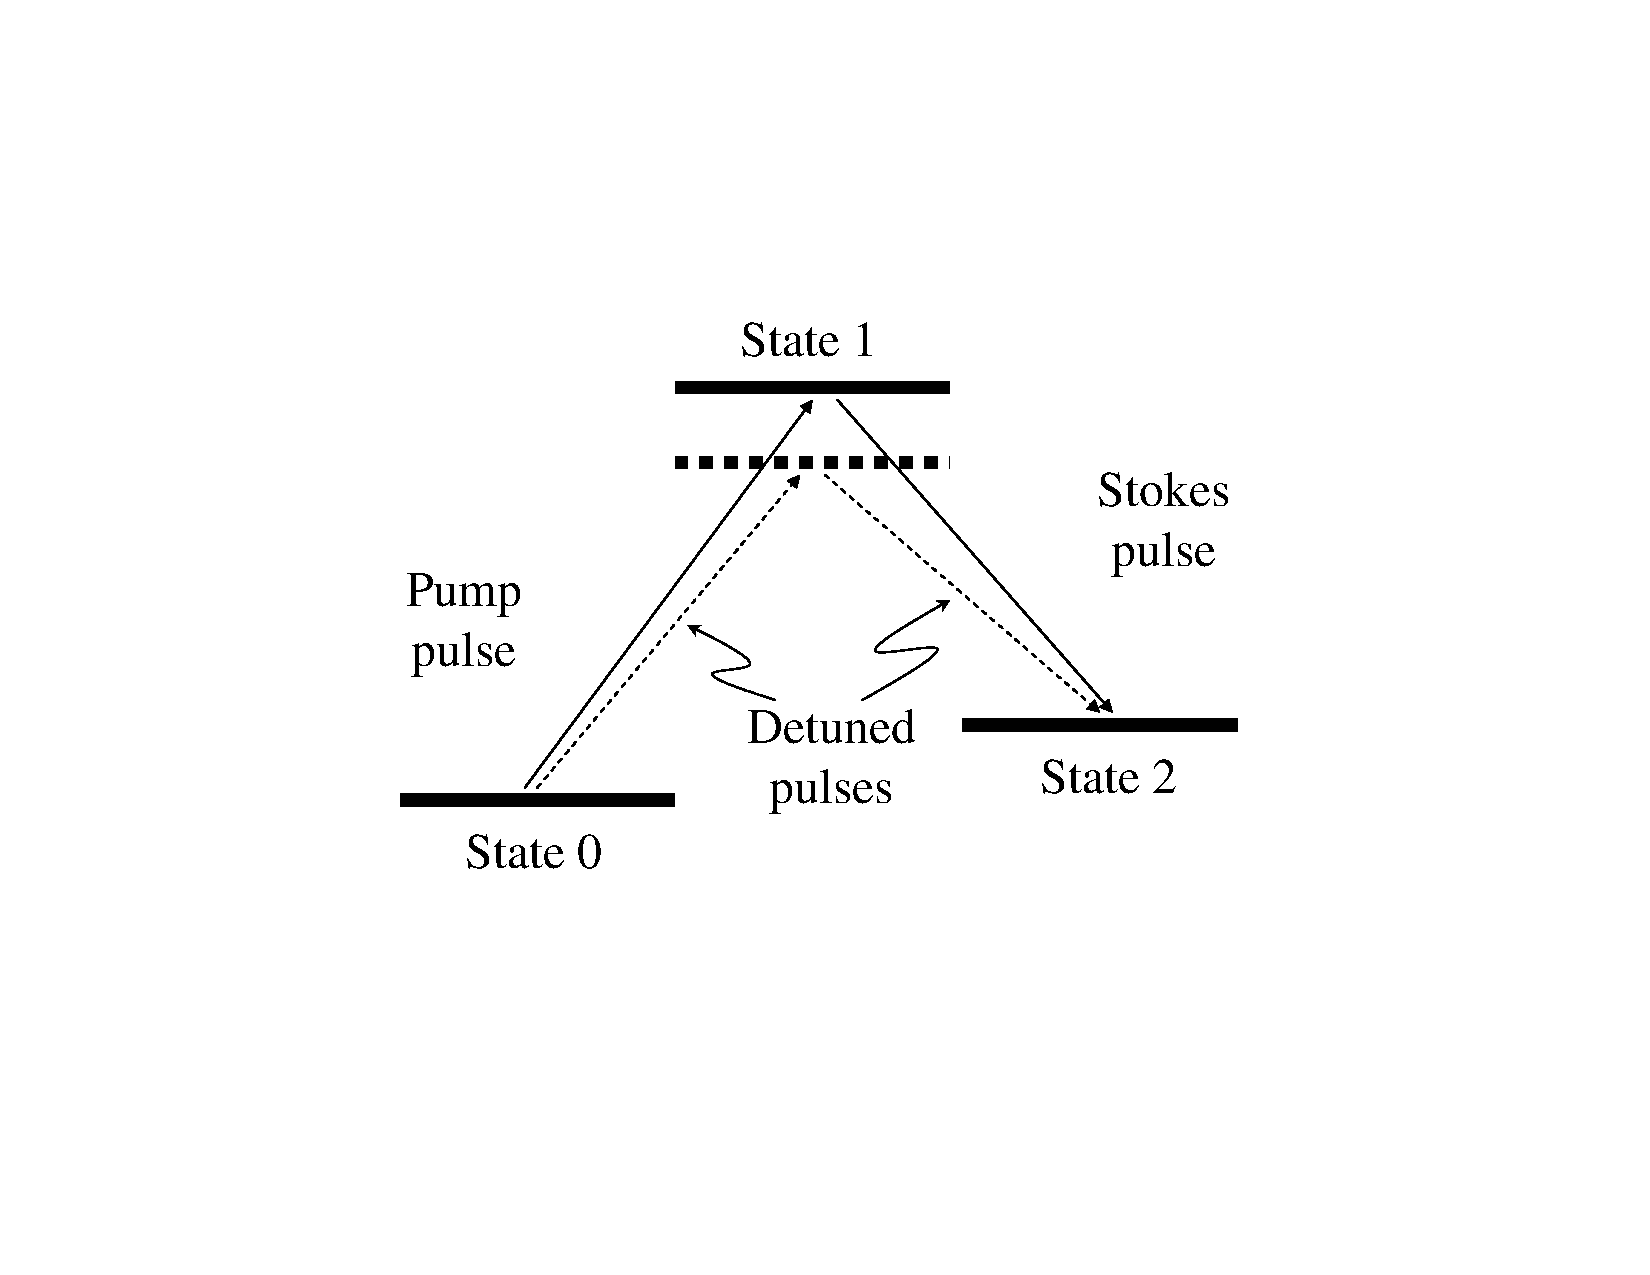
\includegraphics[bb=35 180 489 450]
{sp_detuning/sp_detuning.pdf}
}
\caption[Stokes and pump pulses in a $\Lambda$ system]{Stokes and pump pulses in a $\Lambda$ system. Here we show the pump pulse (connecting states $\ket{0}$ and $\ket{1})$ and the stokes pulse (connecting states $\ket{1}$ and $\ket{2})$. In Figure \ref{amp_surface} we show the effect of amplitude variations on the residue. Also shown here are two \emph{equally} detuned pulses. The figure suggests that significant population will still transfer, but only when the detunings are nearly equal. See Figure \ref{ridge} for an actual calculation.}
\label{sp_detuning}
\end{figure}
%----------------------------------------------------------------------------

%----------------------------------------------------------------------------

To obtain a similar detuning feature for the STIRAP process we start with Equation \ref{dim eom}, obtain equations similar to Equations \ref{doppler eom}, apply the STIRAP pulse sequence, and numerically calculate the inversion probability for various detunings. It is found that (see Figure \ref{ridge}) the detuning feature is a ridge with a long extent along the ridge (roughly fits a Lorentzian with a FWHM of 21.2 inverse cm) and a sharp fall-off along the anti-ridge (roughly fits a Gaussian with a FWHM of 0.424 inverse cm).
%----------------------------------------------------------------------------
%----------------------------------------------------------------------------
%bb defines the bounding box for the pdf
%viewport defines the area of the pdf used
%in sidewaysfigure the last entry in bb moves the caption toward/away the pic
%in sidewaysfigure the second entry in bb moves the pic toward/away the caption
%----------------------------------------------------------------------------
\begin{figure}
\scalebox{0.8}[0.8]{
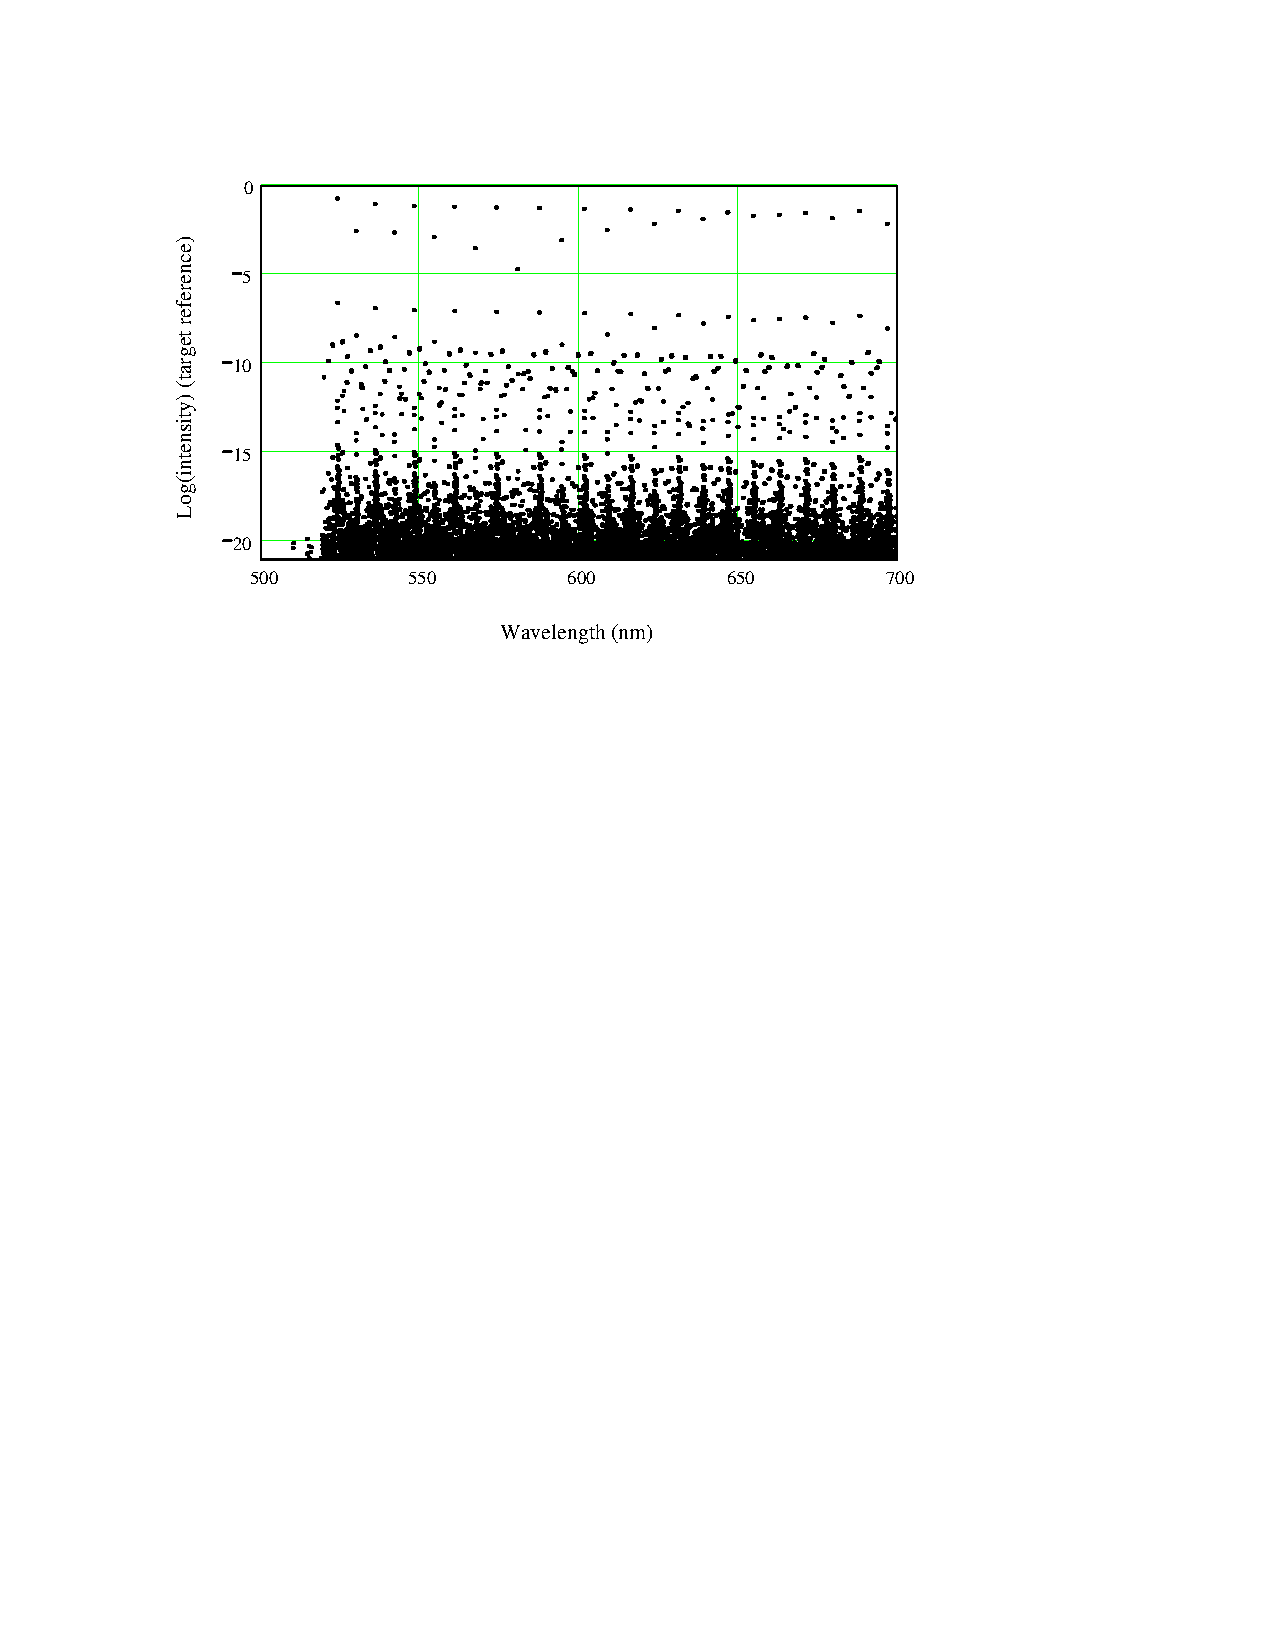
\includegraphics[bb=0 480 489 752]
{PI_79/PI_79.pdf}
}
\caption[Simulated three $\pi$--pulse pathway LIF line strengths (target)]{Simulated three $\pi$--pulse pathway LIF line strengths (target)}
\label{PI_79}
\end{figure}
%----------------------------------------------------------------------------

%----------------------------------------------------------------------------
%bb defines the bounding box for the pdf
%viewport defines the area of the pdf used
%in sidewaysfigure the last entry in bb moves the caption toward/away the pic
%in sidewaysfigure the second entry in bb moves the pic toward/away the caption
%----------------------------------------------------------------------------
\begin{figure}
\scalebox{0.8}[0.8]{
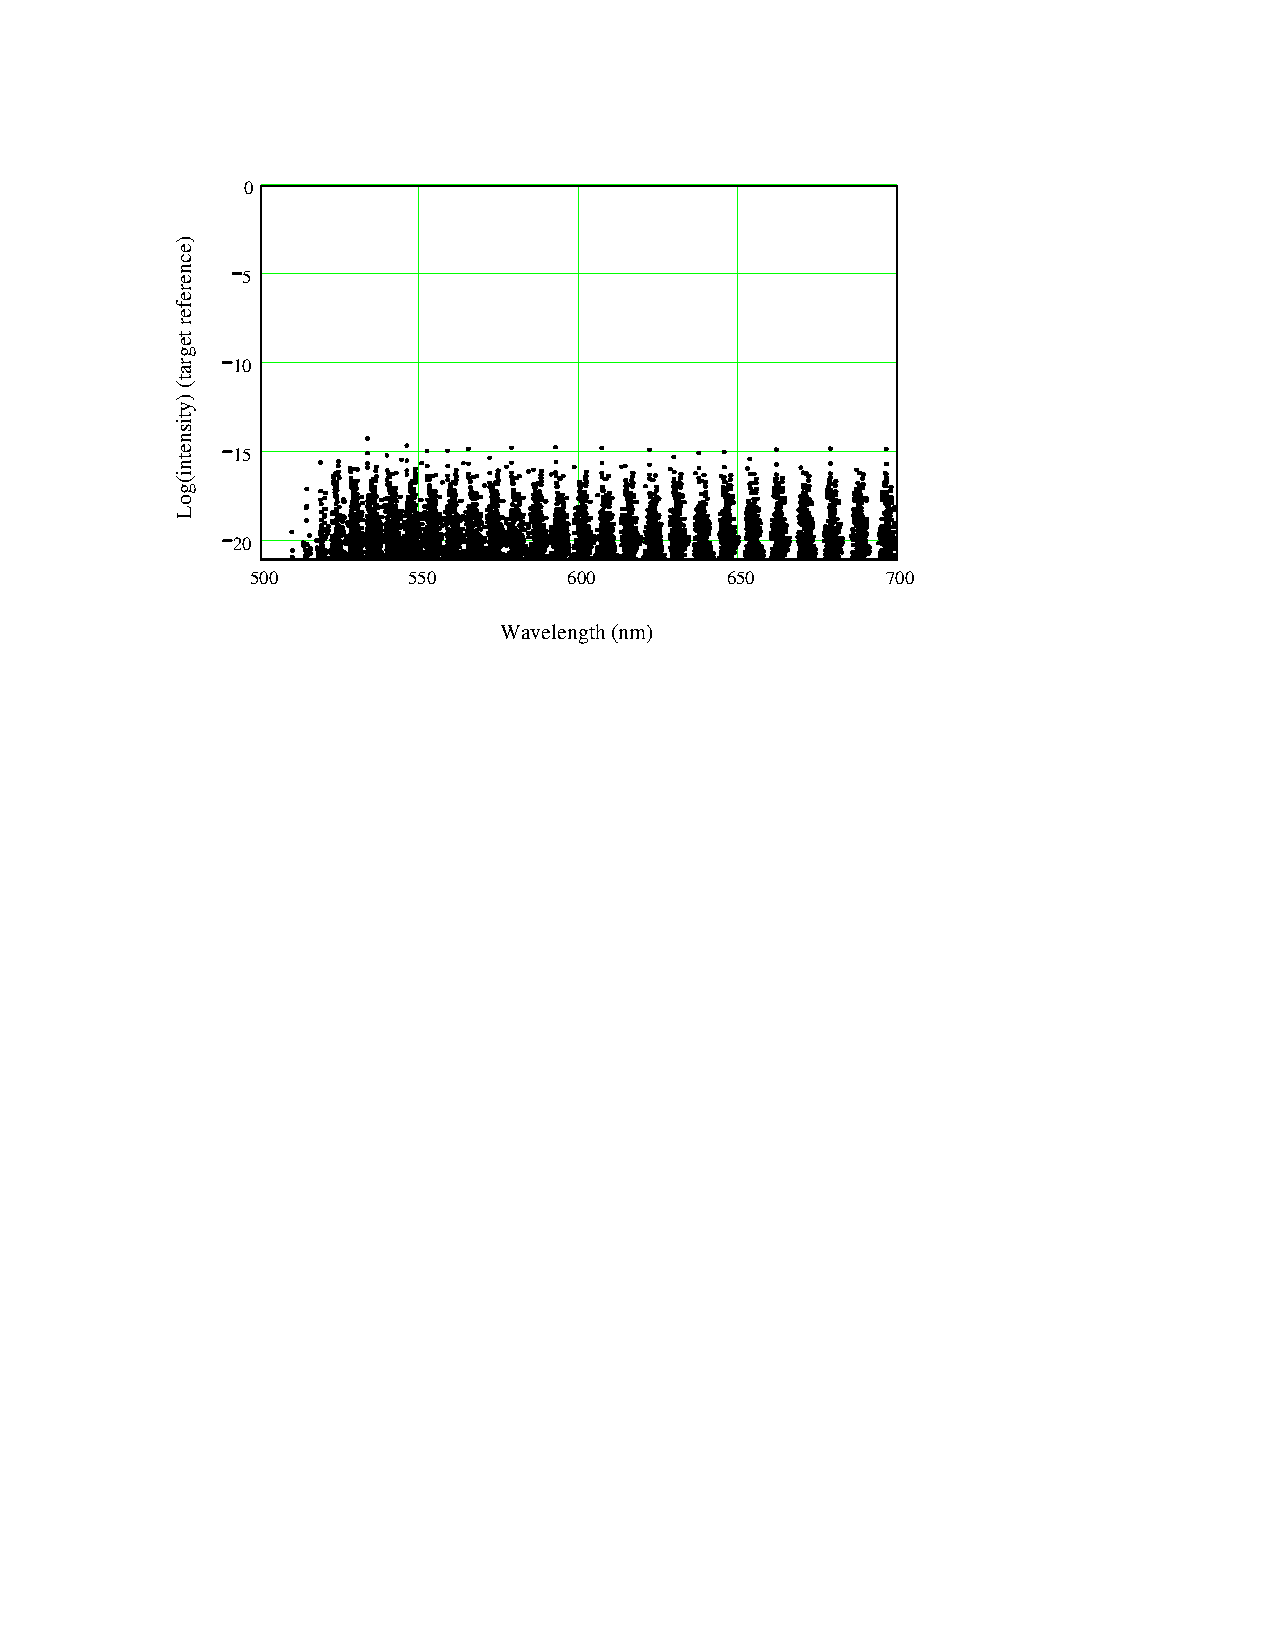
\includegraphics[bb=0 480 489 752]
{PI_77/PI_77.pdf}
}
\caption[Simulated three $\pi$--pulse pathway LIF line strengths (non-target)]{Simulated three $\pi$--pulse pathway LIF line strengths (non-target)}
\label{PI_77}
\end{figure}
%----------------------------------------------------------------------------

%----------------------------------------------------------------------------

To model the effects of this detuning feature of the STIRAP process on the fluorescence spectrum we fit the ridge to an analytic function and use this fit in the computer model described in Section \ref{approx section}. The Lorentzian in Equation \ref{main approx} is replaced with the ridge fit (see Figure \ref{ridge_fit}) and a resulting fluorescence spectrum is calculated.

To compare the STIRAP + $\pi$--pulse (scheme 1) to the three $\pi$--pulse (scheme 2) scheme, we generate plots similar to Figure \ref{target_3}; however, instead of attaching Lorentzian line shapes to each LIF transition we simply plot each transition. See Figure \ref{STIRAP_79} for a plot of the LIF transition supported by scheme 1 for the target molecule, Figure \ref{STIRAP_77} for scheme 1 on the non-target molecule. Compare these plots with Figures \ref{PI_79} and \ref{PI_77} and one sees that scheme 1 ``pulls'' more transitions through the three color pathway than scheme 2. This is one drawback of the robustness of the STIRAP process; however, it does not adversely affect the selectivity of the process since the Lorentzian tail of the fluorescence still dominates (see Figure \ref{target_3} and \ref{non-target_1}).
%----------------------------------------------------------------------------
%----------------------------------------------------------------------------
%bb defines the bounding box for the pdf
%viewport defines the area of the pdf used
%in sidewaysfigure the last entry in bb moves the caption toward/away the pic
%in sidewaysfigure the second entry in bb moves the pic toward/away the caption
%----------------------------------------------------------------------------
\begin{figure}
\scalebox{0.8}[0.8]{
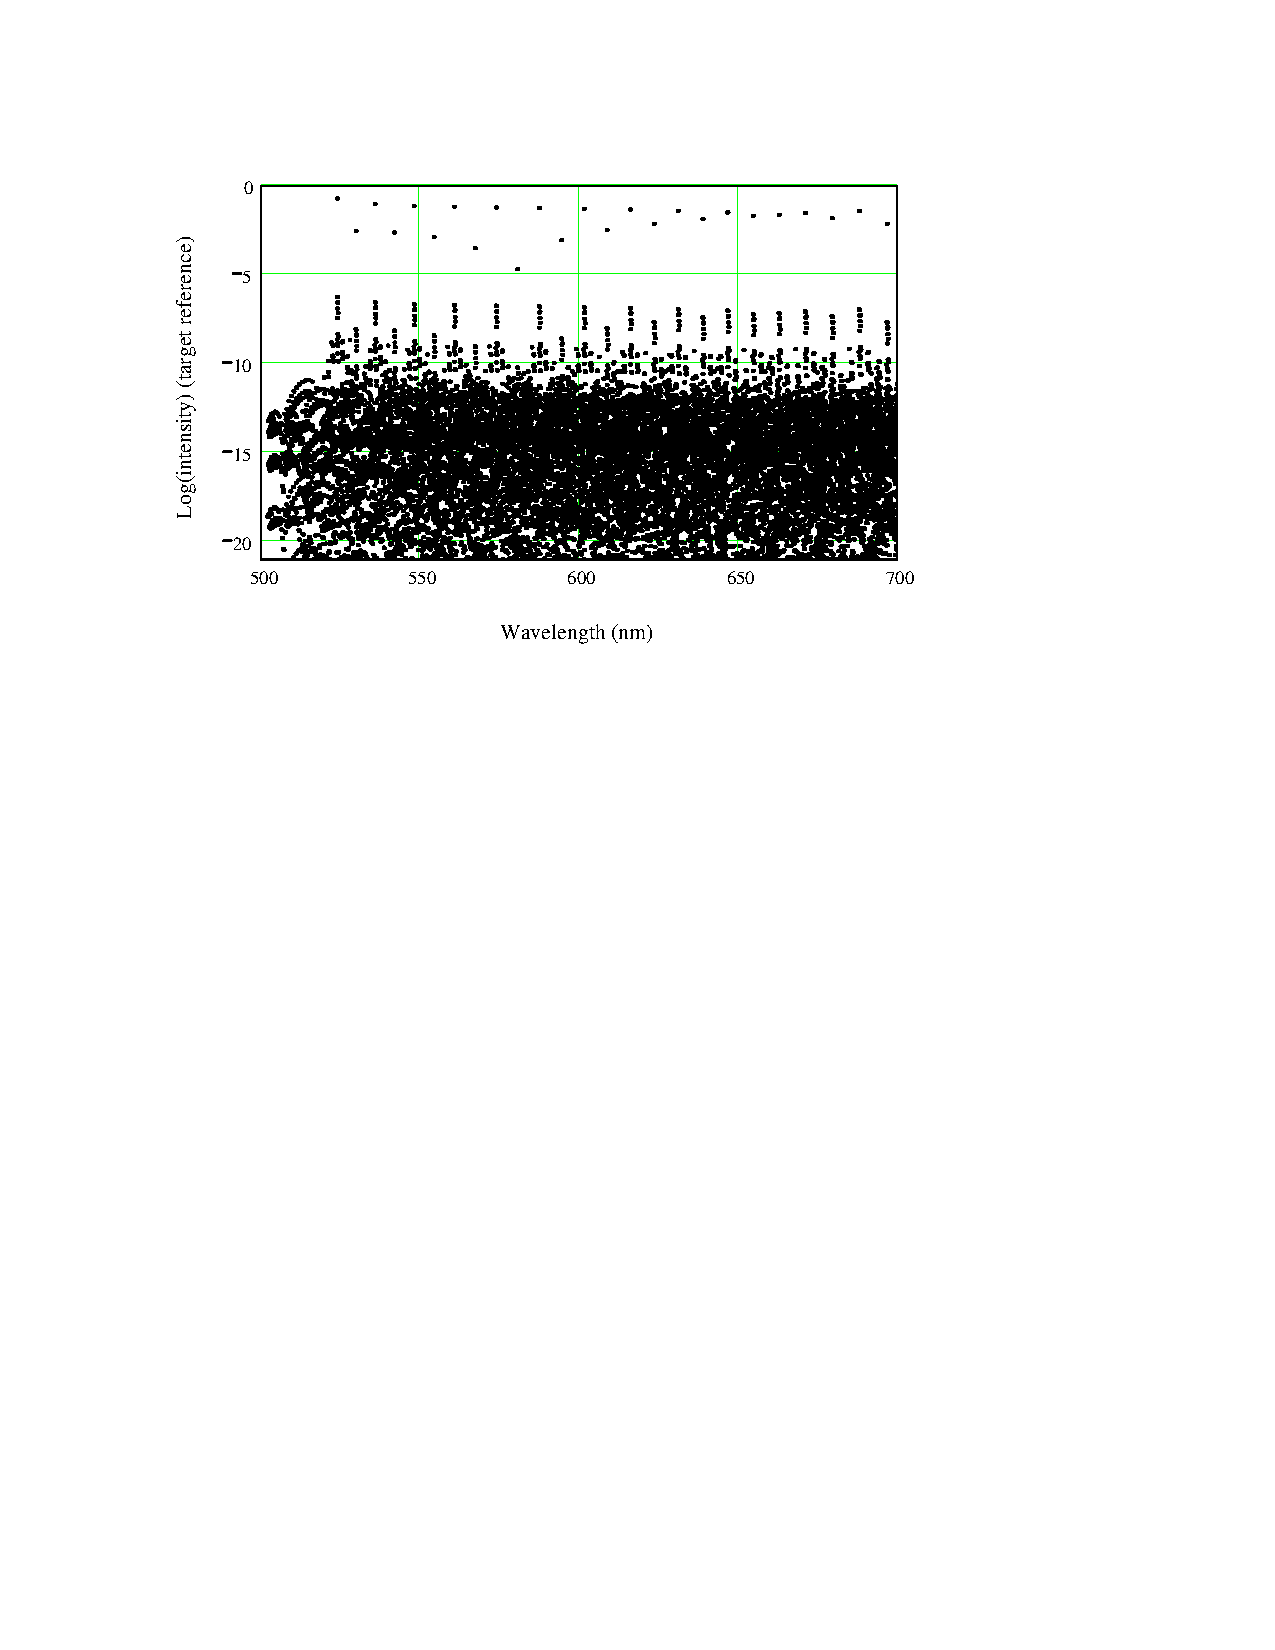
\includegraphics[bb=0 480 489 752]
{STIRAP_79/STIRAP_79.pdf}
}
\caption[Simulated STIRAP + $\pi$--pulse pathway LIF line strengths (target)]{Simulated STIRAP + $\pi$--pulse pathway LIF line strengths (target)}
\label{STIRAP_79}
\end{figure}
%----------------------------------------------------------------------------

%----------------------------------------------------------------------------
%bb defines the bounding box for the pdf
%viewport defines the area of the pdf used
%in sidewaysfigure the last entry in bb moves the caption toward/away the pic
%in sidewaysfigure the second entry in bb moves the pic toward/away the caption
%----------------------------------------------------------------------------
\begin{figure}
\scalebox{0.8}[0.8]{
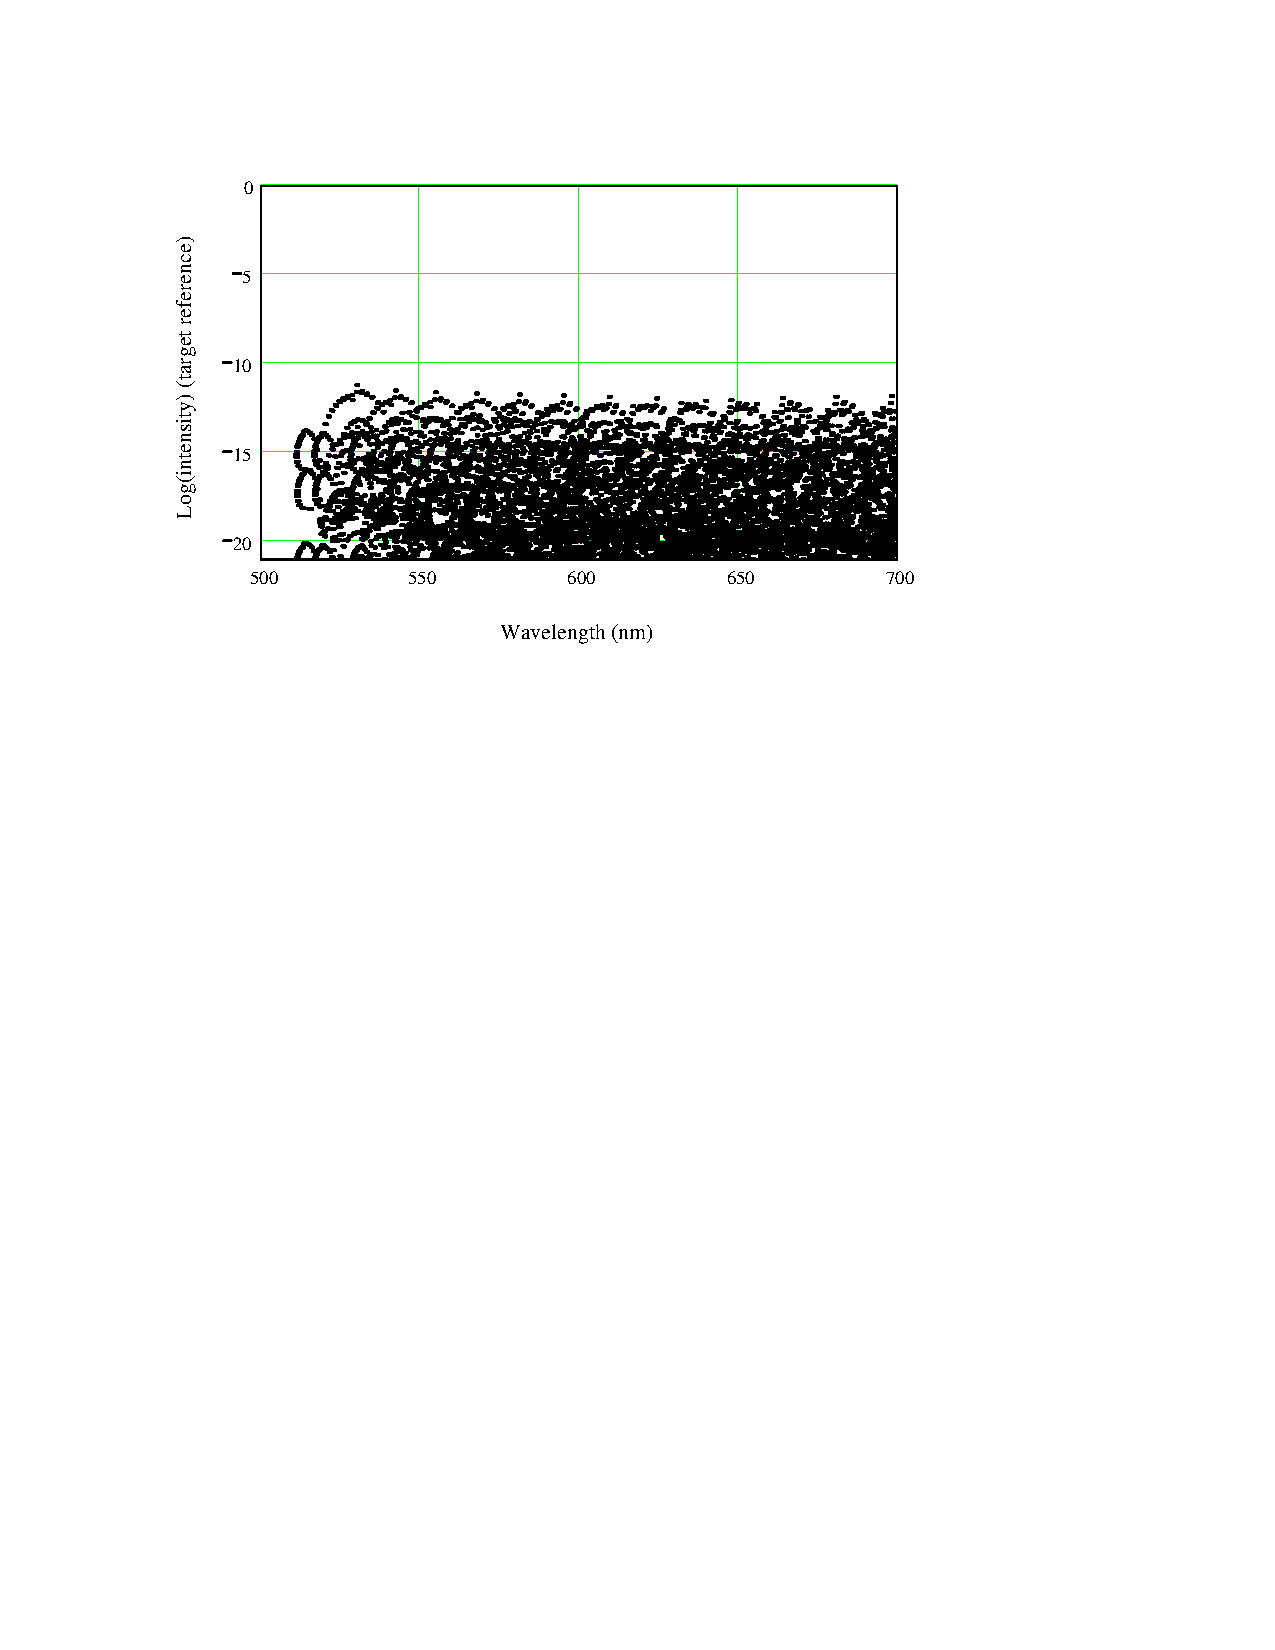
\includegraphics[bb=0 480 489 752]
{STIRAP_77/STIRAP_77.pdf}
}
\caption[Simulated STIRAP + $\pi$--pulse pathway LIF line strengths (non-target)]{Simulated STIRAP + $\pi$--pulse pathway LIF line strengths (non-target)}
\label{STIRAP_77}
\end{figure}
%----------------------------------------------------------------------------

%----------------------------------------------------------------------------
%----------------------------------------------------------------------------
